

\let\negmedspace\undefined
\let\negthickspace\undefined
\documentclass[journal,12pt,twocolumn]{IEEEtran}
%\documentclass[conference]{IEEEtran}
%\IEEEoverridecommandlockouts
% The preceding line is only needed to identify funding in the first footnote. If that is unneeded, please comment it out.
\usepackage{cite}
\usepackage{amssymb,amsfonts,amsthm,amsmath}
\usepackage{algorithmic}
\usepackage{graphicx}
\usepackage{textcomp}
\usepackage{xcolor}
\usepackage{txfonts}
\usepackage{listings}
\usepackage{enumitem}
\usepackage{mathtools}
\usepackage{gensymb}

%%
%\usepackage{setspace}
%%\doublespacing
%\singlespacing
%
%%\usepackage{graphicx}
%%\usepackage{amssymb}
%%\usepackage{relsize}
%\usepackage[cmex10]{amsmath}
%%\interdisplaylinepenalty=2500
%%\savesymbol{iint}
%%\usepackage{txfonts}
%%\restoresymbol{TXF}{iint}
%%\usepackage{wasysym}
%\usepackage{amsthm}
%\usepackage{mathrsfs}
%\usepackage{txfonts}
%%\usepackage{stfloats}
%%\usepackage{cite}
%%\usepackage{cases}
%%\usepackage{subfig}
%%\usepackage{xtab}
%%\usepackage{multirow}
%%\usepackage{algorithm}
%%\usepackage{algpseudocode}
%%\usepackage{tikz}
%%\usepackage{circuitikz}
%%\usepackage{verbatim}
\usepackage{hyperref}
%%\usepackage{stmaryrd}
%%\usepackage{tkz-euclide} % loads  TikZ and tkz-base
%%\usetkzobj{all}
    \usepackage{color}                                            %%
    \usepackage{array}                                            %%
    \usepackage{longtable}                                        %%
    \usepackage{calc}                                             %%
    \usepackage{multirow}                                         %%
    \usepackage{hhline}                                           %%
    \usepackage{ifthen}                                           %%
%  %optionally (for landscape tables embedded in another document): %%
%    \usepackage{lscape}     
%%\usepackage{multicol}
%\usepackage{chngcntr}
%\usepackage{enumerate}

%\usepackage{wasysym}
%\newcounter{MYtempeqncnt}
\DeclareMathOperator*{\Res}{Res}
%\renewcommand{\baselinestretch}{2}
\renewcommand\thesection{\arabic{section}}
\renewcommand\thesubsection{\thesection.\arabic{subsection}}
\renewcommand\thesubsubsection{\thesubsection.\arabic{subsubsection}}

\renewcommand\thesectiondis{\arabic{section}}
\renewcommand\thesubsectiondis{\thesectiondis.\arabic{subsection}}
\renewcommand\thesubsubsectiondis{\thesubsectiondis.\arabic{subsubsection}}

% correct bad hyphenation here
\hyphenation{op-tical net-works semi-conduc-tor}
\def\inputGnumericTable{}                                 %%

\lstset{
language=tex,
frame=single, 
breaklines=true
}

\begin{document}
%


\newtheorem{theorem}{Theorem}[section]
\newtheorem{problem}{Problem}
\newtheorem{proposition}{Proposition}[section]
\newtheorem{lemma}{Lemma}[section]
\newtheorem{corollary}[theorem]{Corollary}
\newtheorem{example}{Example}[section]
\newtheorem{definition}[problem]{Definition}
%\newtheorem{thm}{Theorem}[section] 
%\newtheorem{defn}[thm]{Definition}
%\newtheorem{algorithm}{Algorithm}[section]
%\newtheorem{cor}{Corollary}
\newcommand{\BEQA}{\begin{eqnarray}}
\newcommand{\EEQA}{\end{eqnarray}}
\newcommand{\define}{\stackrel{\triangle}{=}}

\bibliographystyle{IEEEtran}
%\bibliographystyle{ieeetr}


\providecommand{\mbf}{\mathbf}
\providecommand{\pr}[1]{\ensuremath{\Pr\left(#1\right)}}
\providecommand{\re}[1]{\ensuremath{\text{Re}\left(#1\right)}}
\providecommand{\im}[1]{\ensuremath{\text{Im}\left(#1\right)}}
\providecommand{\qfunc}[1]{\ensuremath{Q\left(#1\right)}}
\providecommand{\sbrak}[1]{\ensuremath{{}\left[#1\right]}}
\providecommand{\lsbrak}[1]{\ensuremath{{}\left[#1\right.}}
\providecommand{\rsbrak}[1]{\ensuremath{{}\left.#1\right]}}
\providecommand{\brak}[1]{\ensuremath{\left(#1\right)}}
\providecommand{\lbrak}[1]{\ensuremath{\left(#1\right.}}
\providecommand{\rbrak}[1]{\ensuremath{\left.#1\right)}}
\providecommand{\cbrak}[1]{\ensuremath{\left\{#1\right\}}}
\providecommand{\lcbrak}[1]{\ensuremath{\left\{#1\right.}}
\providecommand{\rcbrak}[1]{\ensuremath{\left.#1\right\}}}
\theoremstyle{remark}
\newtheorem{rem}{Remark}
\newcommand{\sgn}{\mathop{\mathrm{sgn}}}
\providecommand{\abs}[1]{\left\vert#1\right\vert}
\providecommand{\res}[1]{\Res\displaylimits_{#1}} 
\providecommand{\norm}[1]{\left\lVert#1\right\rVert}
%\providecommand{\norm}[1]{\lVert#1\rVert}
\providecommand{\mtx}[1]{\mathbf{#1}}
\providecommand{\mean}[1]{E\left[ #1 \right]}
\providecommand{\fourier}{\overset{\mathcal{F}}{ \rightleftharpoons}}
%\providecommand{\hilbert}{\overset{\mathcal{H}}{ \rightleftharpoons}}
\providecommand{\system}{\overset{\mathcal{H}}{ \longleftrightarrow}}
	%\newcommand{\solution}[2]{\textbf{Solution:}{#1}}
\newcommand{\solution}{\noindent \textbf{Solution: }}
\providecommand{\dec}[2]{\ensuremath{\overset{#1}{\underset{#2}{\gtrless}}}}
\newcommand{\myvec}[1]{\ensuremath{\begin{pmatrix}#1\end{pmatrix}}}
\newcommand{\mydet}[1]{\ensuremath{\begin{vmatrix}#1\end{vmatrix}}}
	\newcommand*{\permcomb}[4][0mu]{{{}^{#3}\mkern#1#2_{#4}}}
\newcommand*{\perm}[1][-3mu]{\permcomb[#1]{P}}
\newcommand*{\comb}[1][-1mu]{\permcomb[#1]{C}}
\providecommand{\gauss}[2]{\mathcal{N}\ensuremath{\left(#1,#2\right)}}
%%
%	%\newcommand{\solution}[2]{\textbf{Solution:}{#1}}
%\newcommand{\solution}{\noindent \textbf{Solution: }}
\newcommand{\cosec}{\,\text{cosec}\,}
\newcommand{\sinc}{\,\text{sinc}\,}
\newcommand{\rect}{\,\text{rect}\,}

%\numberwithin{equation}{section}
\numberwithin{equation}{subsection}
%\numberwithin{problem}{section}
%\numberwithin{definition}{section}
\makeatletter
\@addtoreset{figure}{problem}
\makeatother

\let\StandardTheFigure\thefigure
\let\vec\mathbf
\let\j\jmath
%\renewcommand{\thefigure}{\theproblem.\arabic{figure}}
\renewcommand{\thefigure}{\theproblem}
%\setlist[enumerate,1]{before=\renewcommand\theequation{\theenumi.\arabic{equation}}
%\counterwithin{equation}{enumi}


%\renewcommand{\theequation}{\arabic{subsection}.\arabic{equation}}

\def\putbox#1#2#3{\makebox[0in][l]{\makebox[#1][l]{}\raisebox{\baselineskip}[0in][0in]{\raisebox{#2}[0in][0in]{#3}}}}
     \def\rightbox#1{\makebox[0in][r]{#1}}
     \def\centbox#1{\makebox[0in]{#1}}
     \def\topbox#1{\raisebox{-\baselineskip}[0in][0in]{#1}}
     \def\midbox#1{\raisebox{-0.5\baselineskip}[0in][0in]{#1}}

\vspace{3cm}

\title{
%	\logo{
	Probability: Assignment 5
%	}
}

\author{
	Sree Anusha Ganapathiraju\\
	CC22RESCH11003
	%<-this % stops a space
%\thanks{}}
}

% make the title area
\maketitle

\newpage

%\tableofcontents

\bigskip

\renewcommand{\thefigure}{\theenumi}
\renewcommand{\thetable}{\theenumi}
		\numberwithin{equation}{enumi}
\section{Maximum Likelihood}
\begin{enumerate}[label=\thesection.\arabic*
,ref=\thesection.\theenumi]
\item Generate equiprobable $X \in \cbrak{1,-1}$.\\
\solution\\
The samples are stored in 5\_1.dat file.
\begin{lstlisting}
Assignment 5/codes/equi.py
\end{lstlisting}

\item Generate 
\begin{equation}
Y = AX+N,
\end{equation}
		where $A = 5$ dB,  and $N \sim \gauss{0}{1}$.\\
\solution 
The samples are stored in 5\_2.dat file.
\begin{lstlisting}
Assignment 5/codes/equi.py
\end{lstlisting}
\item Plot $Y$ using a scatter plot.\\
\solution= The code for the plot in Figure \ref{fig:5_3} is below.
\begin{lstlisting}
Assignment 5/codes/equi.py
\end{lstlisting}
\begin{figure}
\centering
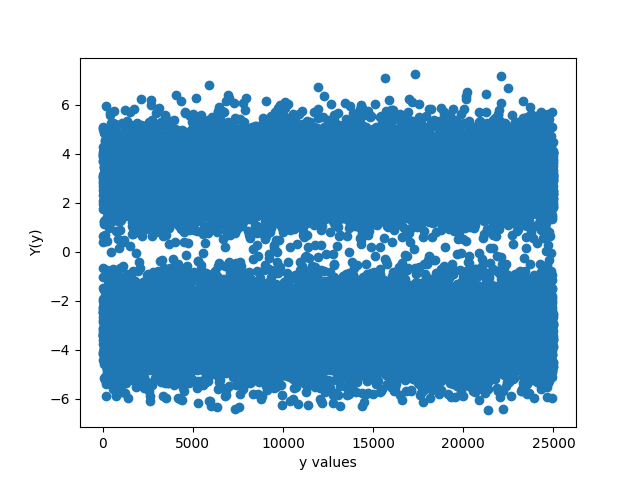
\includegraphics[width=\columnwidth]{./figs/5_3.png}
\caption{The Plot of $Y$}
\label{fig:5_3}
\end{figure}
\item Guess how to estimate $X$ from $Y$.\\
\solution\\
From the plot in Figure \ref{fig:5_3}, we can see that 
\begin{align*}
	\hat{X}&=
	 \begin{cases}
    1 & \text{for Y $<$ 0}\\
      -1 & \text{for Y $>$ 0}
    \end{cases}
 \end{align*}
\item
\label{ml-ch4_sim}
Find 
\begin{equation}
	P_{e|0} = \pr{\hat{X} = -1|X=1}
\end{equation}
and 
\begin{equation}
	P_{e|1} = \pr{\hat{X} = 1|X=-1}
\end{equation}
%
\solution\\
The code for finding the $P_{e|0}$ and $P_{e|1}$ is in
\begin{lstlisting}
Assignment 5/codes/5_5.py
\end{lstlisting}
The values of $P_{e|0}=0.00071$ and $P_{e|1}=0.00081$.
\item Find $P_e$ assuming that $X$ has equiprobable symbols.\\
\solution\\
Using law of total probability, we can find the value of $P_e$,. The value of $P(X=1)=0.5$ and $P(X=-1)=0.5$ as X is equiprobable. 
\begin{align*}
P_e& =P(X=1)\times P_{e|0}+P(X=-1)\times P_{e|1}\\
& = 0.5\times 0.00071 +0.5 \times 0.00081\\
&=0.000355+0.000405\\
&=0.00076\\
&=7.6\times 10^{-4}
\end{align*}
%
\item
Verify by plotting  the theoretical $P_e$ with respect to $A$ from 0 to 10 dB.  \\
\solution\\
\begin{figure}
\centering
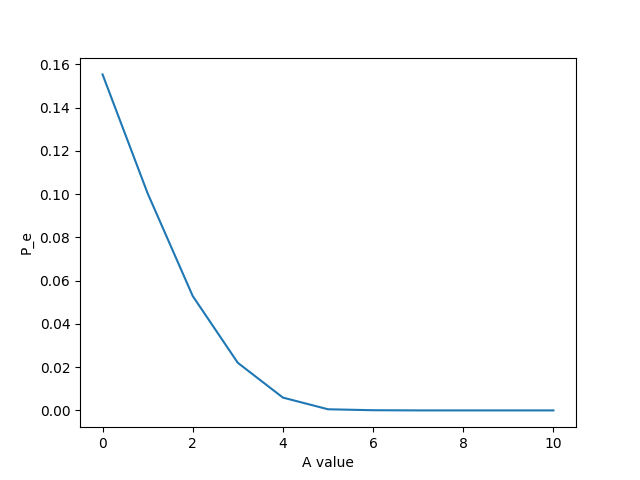
\includegraphics[width=\columnwidth]{./figs/5_6.png}
\caption{The Plot of $P_e$ wrt $A$}
\label{fig:5_6}
\end{figure}
The code for finding thre theoretical $P_e$ wrt $A$ from $0$ to $10$dB is in
\begin{lstlisting}
Assignment 5/codes/5_6.py
\end{lstlisting}
Accoringly, the plot is in Figure \ref{fig:5_6}.
%
\item Now, consider a threshold $\delta$  while estimating $X$ from $Y$. Find the value of $\delta$ that maximizes the theoretical $P_e$.
\item Repeat the above exercise when 
	\begin{align}
		p_{X}(0) = p
	\end{align}
\item Repeat the above exercise using the MAP criterion.

		\end{enumerate}
\end{document}
